\documentclass[pdf, handout]{beamer}
\mode<presentation>{\usetheme{Warsaw}}
%% preamble
 \setbeamertemplate{headline}{}
\setbeamertemplate{section page}[mine]

\setbeamertemplate{footline}[frame number]
% \setbeamertemplate{footline}[]
\title{Valuation of Options - part 3}
\subtitle{Quantitative Finance}
\author{Tilburg University}
\institute{Ramon van den Akker}
\date{}
%%
\usepackage{array}
\usepackage{multirow}
\usepackage{amsmath}
\usepackage{multicol}
\usepackage{subfigure}
\usepackage{graphicx}
\usepackage{pstricks}
\input{commands.txt}
\newcommand{\Var}{\operatorname{Var}}
\renewcommand{\epsi}{\varepsilon}
\newcommand{\argmin}{\mathop{\mathrm{arg\,min}}}
\newcommand{\rank}{\operatorname{rank}}
\renewcommand{\kansp}{\mathbb{P}}
\renewcommand{\calF}{\mathcal{F}}
\newcommand{\e}{\operatorname{e}}
\newcommand{\Bin}{\operatorname{Bin}}
\newcommand{\kbin}{\operatorname{b}}
\newcommand{\lin}{\operatorname{lin}}
\newcommand{\kansq}{\mathbb{Q}}
\DeclareMathOperator*\ster{*} \DeclareMathOperator*\argmax{argmax}
\usepackage{color}
\AtBeginSection{\frame{\sectionpage}}
\newtranslation[to=greek]{Section}{En'othta}
\newtranslation[to=greek]{Subsection}{Upoen'othta}
\defbeamertemplate{section page}{mine}[1][]{%
  \begin{centering}
    {\usebeamerfont{section name}\usebeamercolor[fg]{section name}#1}
    \vskip1em\par
    \begin{beamercolorbox}[sep=12pt,center]{part title}
      \usebeamerfont{section title}\insertsection\par
    \end{beamercolorbox}
  \end{centering}
}
\defbeamertemplate{subsection page}{mine}[1][]{%
  \begin{centering}
    {\usebeamerfont{subsection name}\usebeamercolor[fg]{subsection name}#1}
    \vskip1em\par
    \begin{beamercolorbox}[sep=8pt,center,#1]{part title}
      \usebeamerfont{subsection title}\insertsubsection\par
    \end{beamercolorbox}
  \end{centering}
}

\begin{document}

% title frame
\begin{frame}
\titlepage
\end{frame}

\begin{frame}{Assumptions  Black-Scholes market (recap)}
In class we will almost exclusively work with the `Black-Scholes market'.
\\ \vspace{.5cm}
\textbf{Assumptions on price processes:} \\
Asset price:
\[
\rd S_t=\mu S_t \rd t + \sigma S_t \rd W_t,\quad S_0=s_0,\,\,\, \var(W_1) = 1
\]
Money Market Account:
\[
\rd B_t= r B_t \rd t,\quad B_0=1
\]
\textbf{Assumptions on market:} \\
\begin{itemize}
\item frictionless trading
\begin{itemize}
\item no transaction costs
\item trading in continuous-time is possible
\item no restrictions on short sales and fractional positions
\end{itemize}
\item no credit/counterparty risk: borrowing rate = lending rate
\end{itemize}
\end{frame}

\begin{frame}{Agenda}
\begin{itemize}
\item we are interested in the price $C_t$, for $t\in [0,T)$, of (European) option with payoff $h(S_T)$ at expiration date/maturity $T$
\item we will discuss three methods to determine fair price (using continuous-time model for financial market):
\begin{itemize}
\item Black-Scholes Partial Differential Equation
\item risk-neutral pricing
\item pricing kernel
\end{itemize}
\textbf{These slides discuss risk neutral pricing and the pricing kernel approach.} 
\end{itemize}
\end{frame}


\section{Risk-neutral pricing}

\begin{frame}{Motivation}
We have proved the First Fundamental Theorem of asset pricing for the toy model (see part 1). Now we will  state the continuous-time version.
\end{frame}


%Recall from Part 1: \\
%\vspace{.25cm}
%\textbf{First fundamental theorem (risk-neutral version) for  single period}: \\
%absence of arbitrage holds
%if and only if
%for a chosen num\'{e}raire $N$ and a probability measure $\mathbb{Q}$ \emph{equivalent} to
%$\mathbb{P}$ we have for any asset with price $S$:
%\[
%\frac{S_0}{N_0}=\mathbb{E}_{\mathbb{Q}} \frac{S_1}{N_1}
%\]
%\textbf{Remark:}
%\begin{itemize}
%\item for $N=B$ we have
%\[
%\mathbb{E}_{\mathbb{Q}} \frac{S_1}{S_0}=\frac{B_1}{B_0}
%\]
%$\implies$ under $\mathbb{Q}$: no reward for taking risk $\implies$ risk-neutral
%\end{itemize}
%\end{frame}
%%
%\begin{frame}[toc=]{Motivation - relation to pricing kernel}
%\vspace{-.7cm}
%\small{
%\[
%\frac{S_0}{N_0}=\mathbb{E}_{\mathbb{Q}} \frac{S_1}{N_1}
%\]
%\vspace{-.3cm}
%\begin{itemize}
%\item where does the equivalent measure $\mathbb{Q}$ come from?
%\item we have
%\[
%S_0=N_0\mathbb{E}_{\mathbb{Q}} \frac{S_1}{N_1}=N_0\int \frac{S_1}{N_1} (\omega) \rd\mathbb{Q}(\omega)
%= N_0\int \frac{S_1}{N_1} (\omega) \frac{ \rd \mathbb{Q}}{\rd\mathbb{P}}(\omega) \rd\mathbb{P}(\omega)
%\]
%\item by pricing kernel version of  FFT we have
%\[
%S_0=\mathbb{E}_{\mathbb{P}} m S_1 =\int m (\omega) S_1(\omega) \rd\mathbb{P}(\omega)
%\]
%So\vspace{-.15cm}
%\[
%\frac{ \rd \mathbb{Q}}{\rd\mathbb{P}}= m \frac{N_1}{N_0}
%\]
%and $\mathbb{Q}$ is determined by, for all events $A$,
%\vspace{-.2cm}
%\[
%\mathbb{Q}(A)=\mathbb{E}_{\mathbb{P}} 1_A \frac{ \rd \mathbb{Q}}{\rd\mathbb{P}}
%\]
%\end{itemize}
%}
%%usually specified by Radon-Nikodym derivative $\theta=\rd\mathbb{Q}/\rd \mathbb{P}$: a random variable
%%with $\theta>0$ and for any random variable $X$:
%%\[
%%\mathbb{E}_{\mathbb{Q}} X=\mathbb{E}_{\mathbb{P}} \theta X.
%%\]
%%Symbolic intuition:
%%\[
%%\mathbb{E}_{\mathbb{Q}} X=\int X \rd\mathbb{Q}=\int  X \frac{\rd \mathbb{Q}}{\rd \mathbb{P}}\rd\mathbb{P}
%%=\mathbb{E}_{\mathbb{P}} \theta X
%%\]
%%\textbf{Remark:} \\
%%the set of all probability measures equivalent to $\mathbb{P}$ is determined by
%%\begin{itemize}
%%\item $\theta>0$
%%\item $\mathbb{E}_{\mathbb{P}} \theta=1$
%%\end{itemize}}
%\end{frame}

%
\begin{frame}{The First Fundamental Theorem of asset pricing}
%\vspace{-.25cm}
\begin{theorem} Under regularity conditions: 
absence of arbitrage holds if and only if,
for some num\'{e}raire $N$, there exists a probability measure $\mathbb{Q}=\mathbb{Q}_N$ such that:
\begin{itemize}
\item[(1)] $\mathbb{Q}$ is equivalent to $\mathbb{P}$;
\begin{itemize}
\item i.e. $\mathbb{Q}(A)>0$ iff $\mathbb{P}(A)>0$ and $\mathbb{Q}(A)=0$ iff $\mathbb{P}(A)=0$;
\end{itemize}
\item[(2)] for any asset $A$ in the market: the discounted price process $A/N$ is a $\mathbb{Q}$-martingale, i.e. 
\[
\frac{A_t}{N_t}=\mathbb{E}_{\mathbb{Q}}\left[ \frac{A_{t+h}}{N_{t+h}} \mid \calF_t \right] 
=
\mathbb{E}_{\mathbb{Q}}\left[ \frac{A_{T}}{N_{T}} \mid \calF_t \right].
\]
\end{itemize}
%\textbf{Theorem} \\
%if there is \emph{No Free Lunch Without Vanishing Risk}  there exists probability measure $\mathbb{Q}$ such that (1)-(2) hold
%\begin{itemize}
%\item NFLWVR is rather subtle relaxation of no-arbitrage which is (far) beyond (technical) scope of QF
%\item you are allowed to read the theorems as an ``if and only if''
%\end{itemize}
\end{theorem}
\textbf{Remarks:}
\begin{itemize}
\item any traded asset $A$ with $\mathbb{P}(A_t > 0)=1$ for all $t$ can be used as num\'{e}raire
\item typically the Money Market Account $B$ is used as num\'{e}raire 
\end{itemize}
%
\end{frame}
%
\begin{frame}{Proof}
We will only give a full proof for the Black-Scholes market. To prepare for the proof we first notice the following:
\begin{itemize}
\item Consider Black-Scholes market
\item Use $N=B$
\item If $V$ is self-financing portfolio then
\begin{align*}
\rd \frac{V_t}{B_t}
&= \frac{1}{B_t} \rd V_t - r \frac{V_t}{B_t}  
\rd t =
\frac{1}{B_t}(\phi_t \rd S_t + \psi_t \rd B_t)
 -r \frac{V_t}{B_t} \rd t \\
 & =\dots = \phi_t \rd \frac{S_t}{B_t}
\end{align*}
Hence: if $S/B$ is $\mathbb{Q}$-martingale, then
$V/B$ is $\mathbb{Q}$-martingale as well!
\end{itemize}
\end{frame}


\begin{frame}{First Fundamental Theorem of asset pricing}
\begin{proof} `$\Leftarrow$' (general proof; not only for Black-Scholes market)
\begin{itemize}
\item let $V$ be the value process corresponding to a self-financing trading strategy
\item suppose $V$ satisfies $\mathbb{P}(V_T < 0 ) =0$ and $\mathbb{P}(V_T>0) >0$
\begin{itemize}
\item if $\mathbb{P}(V_0 \leq 0)=1$ we would have an arbitrage opportunity
\end{itemize}
\item equivalence yields: $\mathbb{Q}(V_T < 0 ) =0$ and $\mathbb{Q}(V_T>0) >0$
\item we have (use previous slide!)
\[
V_0 = N_0 \mathbb{E}_\mathbb{Q} \left[  \frac{V_T}{N_T} \mid \calF_0 \right]
=N_0 \mathbb{E}_\mathbb{Q} \left[  \frac{V_T}{N_T}  \right] >0
\]
\item consequently $\mathbb{P}(V_0>0)>0$ $\implies$ strategy does not yield arbitrage opportunity 
\end{itemize}
`$\Rightarrow$' We do not prove this implication in general. For the Black-Scholes market you will see an 'explicit' construction.
\end{proof}
\end{frame}

\begin{frame}{Using the first fundamental theorem to price options}
\begin{itemize}
\item[(a)] Construct model for basic assets (for example, $S$ and $B$).
\item[(b)] Apply FFT: If your model does not allow for arbitrage opportunities, FFT says that you should be able to find $\mathbb{Q}\sim\mathbb{P}$ such that $S/B$ is $\mathbb{Q}$-martingale (assuming that you use $B$ as num\'{e}raire, note that $B/B$ then yields a martingale).
Use this to determine $\mathbb{Q}$. We will (typically) find unique solution.
\item[(c)] Now introduce an option (on $S$) to the market. We know its payoff $h(S_T)$ at maturity and
want to determine its no-arbitrage price $C_t$ for $t<T$.
\item[(d)] Apply FFT: $B/N$, $S/N$, and $C/N$ should be $\mathbb{Q}$-martingales.
From step (b) you already obtained unique $\mathbb{Q}$. 
This implies that we must set price of option $C_t$, for $t\in [0, T)$, via
\begin{align*}
C_t &=  N_t \mathbb{E}_{\mathbb{Q}}\left[ 
\frac{C_T}{N_T} \mid \mathcal{F}_t
\right] = N_t \mathbb{E}_{\mathbb{Q}}\left[ 
\frac{h(S_T)}{N_T} \mid \mathcal{F}_t
\right].
\end{align*}
%\item[(d)] Assume that we can find
%self-financing portfolio $V$ replicating  payoff of option at maturity, i.e. %$V_T=C_T$. Later on we show that
%this assumption is always satisfied in the B-S market.
%\item[(e)] As the replicating portfolio is self-financing, we
%must have $C_t=V_t$ (otherwise arbitrage opportunities would exist). 
%Combining the previous results yields
\end{itemize}
\end{frame}



\begin{frame}{Using the first fundamental theorem to price option}
\begin{itemize}
\item price processes basic assets in standard Black-Scholes market given; in particular: 
\[
S_T = S_t \exp\left(  (\mu - \frac{1}{2}\sigma^2)(T-t) + \sigma (W_T^{\mathbb{P}} - W_t^{\mathbb{P}})   \right),
\]
where $W^{\mathbb{P}}$ is a standard $\mathbb{P}$-Brownian motion
\item use these to solve for $\mathbb{Q}$
\begin{itemize}
\item \textbf{\color{red}{how?}  }
\end{itemize}
\item want to price European option with payoff $C_T=h(S_T)$:
\[
C_t=N_t \mathbb{E}_{\mathbb{Q}}\left[ \frac{C_T}{N_T} \mid \mathcal{F}_t  \right]
=N_t \mathbb{E}_{\mathbb{Q}}\left[ \frac{h(S_T)}{N_T} \mid \mathcal{F}_t  \right]
\]
\begin{itemize}
\item in case $N_t=B_t=\exp(rt)$:
\[
C_t=\e^{-r(T-t)} \mathbb{E}_{\mathbb{Q}}\left[  C_T \mid \mathcal{F}_t  \right]
=\e^{-r(T-t)} \mathbb{E}_{\mathbb{Q}}\left[  h(S_T) \mid \mathcal{F}_t  \right]
\]
\end{itemize}
\item $\implies$
\textbf{\color{red}{we do not need to know $\mathbb{Q}$, but `only' need to know the distribution of $W^{\mathbb{P}}$, and hence $S_T$,  under $\mathbb{Q}$!}}
\end{itemize}

\end{frame}
%
\begin{frame}{Intermezzo: Girsanov}
\begin{theorem}[Girsanov]
\small{
Suppose the process $W^{\mathbb{P}}$ is a standard Brownian motion under $\mathbb{P}$ and  let $T<\infty$.
Consider a process $(\gamma_t)_{t\geq 0}$  adapted to the filtration $(\mathcal{F}_t)_{t\geq 0}$  generated by $W^{\mathbb{P}}$ and
satisfying appropriate integrability conditions.
Define
% a new process $(\theta_t)_{t\geq 0}$ by $\theta_0=1$ and the SDE
%\[
%\rd \theta_t=-\gamma_t \theta_t \rd W^{\mathbb{P}}_t.
%\]
%Then 
$\mathbb{Q}$ by, for events $A \in\mathcal{F}_T$,
\[
\mathbb{Q}(A)=%\mathbb{E}_{\mathbb{P}}\left[  \theta_T \right]=
\mathbb{E}_{\mathbb{P}}\left[ 1_A \exp\left(  -\frac{1}{2} \int_0^T \gamma_t^2 \rd t   - \int_0^T \gamma_t  \rd W^{\mathbb{P}}_t         \right)\right].
\]
Then we have:
\begin{itemize}
\item
$\mathbb{Q}$ is a probability measure equivalent to $\mathbb{P}$,
\item and the process $W^{\mathbb{Q}}$ defined by
\[
W^{\mathbb{Q}}_0=0,\quad
\rd W^{\mathbb{Q}}_t=\gamma_t \rd t + \rd W^{\mathbb{P}}_t 
,
\]
or equivalently $
W^{\mathbb{Q}}_t=\int_0^t \gamma_u \rd u +  W^{\mathbb{P}}_t$,
is a standard Brownian motion under $\mathbb{Q}$.
\end{itemize}
}
\end{theorem}
%\textbf{Remark:} $W^{\mathbb{Q}}$ is \textbf{not} a standard
%Brownian motion under $\mathbb{P}$
\end{frame}
%
\begin{frame}{Intermezzo: Girsanov}
\begin{figure}
\mbox{
 \subfigure{
 \includegraphics[height=0.49\textwidth]{Girsanov_left.eps} } \quad
      \subfigure{{\includegraphics[width=0.4\textwidth]{Girsanov_right.eps}}}
}
\end{figure}
\begin{itemize}
\item source: Wikipedia
\item under $\mathbb{Q}$ and $\mathbb{P}$ same sample paths possible (equivalence), but with different likelihoods
\end{itemize}
\end{frame}

\begin{frame}{Sketch proof Girsanov}
\begin{itemize}
\item given the integrability conditions, it is easy to show that $\mathbb{Q}$ is probability measure equivalent to $\mathbb{P}$
\item to prove that $W^{\mathbb{Q}}$ is a standard Brownian motion under $\mathbb{Q}$ we need to show, for any $0=t_0<t_1<\dots<t_n\leq T$, that
\[
(W_{t_1}^{\mathbb{Q}} - W_{t_0}^{\mathbb{Q}},\dots,W_{t_n}^{\mathbb{Q}} - W^{\mathbb{Q}}_{t_{n-1}})\distr N(0_n, \Sigma)
\]
where $\Sigma_{ij}=0$ for $i\neq j$ 
and $\Sigma_{ii} = t_i -t_{i-1}$
\item we only consider case in which $u\mapsto \gamma_u$ is deterministic and  $n=2$ with $t_2=T$
\item it is sufficient to show (MGF determines the probability distribution)
\[
\mathbb{E}_{\mathbb{Q}}\left[ \e^{a_1 (W^{\mathbb{Q}}_{t_1} - W^{\mathbb{Q}}_{t_0}) + a_2 (W^{\mathbb{Q}}_{t_2} - W^{\mathbb{Q}}_{t_1})}\right]  = \e^{\frac{1}{2}\left(a_1^2(t_1-t_0) + a_2^2(t_2-t_1)
\right)} 
\]
\end{itemize}
\end{frame}

\begin{frame}{Sketch proof Girsanov}
We  have 
\begin{align*}
&\mathbb{E}_{\mathbb{Q}}\left[ \e^{a_1 (W_{t_1}^{\mathbb{Q}} - W_{t_0}^{\mathbb{Q}}) + a_2 (W^{\mathbb{Q}}_{t_2} - W^{\mathbb{Q}}_{t_1})}\right]= 
\mathbb{E}_{\mathbb{P}}\left[\frac{\rd\mathbb{Q}}{\rd\mathbb{P}} \e^{a_1 (W_{t_1}^{\mathbb{Q}} - W^{\mathbb{Q}}_{t_0}) + a_2 (W^{\mathbb{Q}}_{t_2} - W^{\mathbb{Q}}_{t_1})}\right] \\
 &\quad=
\mathbb{E}_{\mathbb{P}}\left[
\e^{a_1 (W^{\mathbb{Q}}_{t_1} - W^{\mathbb{Q}}_{t_0}) + a_2 (W^{\mathbb{Q}}_{t_2} - W^{\mathbb{Q}}_{t_1})}
\e^{-\frac{1}{2}\int_0^T \gamma_u^2 \rd u - \int_0^T \gamma_u \rd W^{\mathbb{P}}_u}
\right] \\
 &\quad=
\e^{
a_1 \int_{t_0}^{t_1} \gamma_u \rd u + a_2 \int_{t_1}^{t_2} \gamma_u \rd u 
-\frac{1}{2}\int_{t_0}^{t_2} \gamma_u^2  \rd u} \\
&\qquad\quad \times
\mathbb{E}_{\mathbb{P}}\left[
\e^{ 
-\int_{t_0}^{t_1} ( \gamma_u - a_1)  \rd W^{\mathbb{P}}_u
-\int_{t_1}^{t_2} (\gamma_u - a_2)  \rd W^{\mathbb{P}}_u
}
\right]
\end{align*}
Exploiting independent increments and  
$\int_a^b f_u \rd W^{\mathbb{P}}_u \distr N( 0, \int_a^b f_u^2 \rd u)$ for deterministic functions $f$:
\begin{align*}
& \mathbb{E}_{\mathbb{P}}\left[
\e^{ 
-\int_{t_0}^{t_1} ( \gamma_u - a_1)  \rd W^{\mathbb{P}}_u
-\int_{t_1}^{t_2} (\gamma_u - a_2)  \rd W^{\mathbb{P}}_u
}
\right] \\
&\quad =
\mathbb{E}_{\mathbb{P}}
\left[
\e^{ 
-\int_{t_0}^{t_1} ( \gamma_u - a_1)  \rd W^{\mathbb{P}}_u }
\right]
\mathbb{E}_{\mathbb{P}}
\left[\e^{ 
-\int_{t_1}^{t_2} ( \gamma_u - a_2)  \rd W^{\mathbb{P}}_u}\right]
\\
&\quad
= \e^{
\frac{1}{2} \int_{t_0}^{t_1} ( \gamma_u - a_1)^2 \rd u
}\e^{
\frac{1}{2} \int_{t_1}^{t_2} ( \gamma_u - a_2)^2 \rd u
}  = \e^{\frac{1}{2}\int_{t_0}^{t_2} \gamma_u^2 \rd u 
- a_1 \int_{t_0}^{t_1} \gamma_u \rd u 
- a_2 \int_{t_1}^{t_2} \gamma_u \rd u
} \\
&\qquad \times \e^{\frac{1}{2}\left( a_1^2 (t_1-t_0) + a_2^2 (t_2- t_0)\right)
} \text{ which yields the result}
\end{align*}
\end{frame}


\begin{frame}{Remarks}
\vspace{-.7cm}
\begin{itemize}
\item Girsanov: for
\[
W^{\mathbb{Q}}_0=0,\quad
\rd W^{\mathbb{Q}}_t=\gamma_t \rd t + \rd W^{\mathbb{P}}_t\quad ( W^{\mathbb{P}} \text{ standard BM  under } \mathbb{P} )
\]
we can find $\mathbb{Q}$ equivalent to $\mathbb{P}$ such that 
$W^{\mathbb{Q}}$
is  standard Brownian motion under $\mathbb{Q}$ 
\item Let $0<a\neq 1$. Suppose that we can find probability measure
$\mathbb{Q}$ such that
\[
Z^{\mathbb{Q}}_0=0,\quad
\rd Z^{\mathbb{Q}}_t=\gamma_t \rd t + a \rd W^{\mathbb{P}}_t\quad ( W^{\mathbb{P}} \text{ standard BM  under } \mathbb{P} ),
\]
is standard Brownian motion under $\mathbb{Q}$.
Then $\mathbb{Q}$ is \emph{not} equivalent to $\mathbb{P}$.
\end{itemize}
\end{frame}

\begin{frame}{Back to valuation: exploiting Girsanov}
%\vspace{-.25cm}
\begin{theorem} Under regularity conditions: 
absence of arbitrage holds if and only if,
for some num\'{e}raire $N$, there exists a probability measure $\mathbb{Q}=\mathbb{Q}_N$ such that:
\begin{itemize}
\item[(1)] $\mathbb{Q}$ is equivalent to $\mathbb{P}$;
\begin{itemize}
\item i.e. $\mathbb{Q}(A)>0$ iff $\mathbb{P}(A)>0$ and $\mathbb{Q}(A)=0$ iff $\mathbb{P}(A)=0$;
\end{itemize}
\item[(2)] for any price process $A$ in the market, the discounted price process $A/N$ is a $\mathbb{Q}$-martingale, i.e. 
\[
\frac{A_t}{N_t}=\mathbb{E}_{\mathbb{Q}}\left[ \frac{A_{t+h}}{N_{t+h}} \mid \calF_t \right] 
=
\mathbb{E}_{\mathbb{Q}}\left[ \frac{A_{T}}{N_{T}} \mid \calF_t \right].
\]
\end{itemize}
%\textbf{Theorem} \\
%if there is \emph{No Free Lunch Without Vanishing Risk}  there exists probability measure $\mathbb{Q}$ such that (1)-(2) hold
%\begin{itemize}
%\item NFLWVR is rather subtle relaxation of no-arbitrage which is (far) beyond (technical) scope of QF
%\item you are allowed to read the theorems as an ``if and only if''
%\end{itemize}
\end{theorem}
\textbf{Remarks:}
\begin{itemize}
\item any asset $A$ with $\mathbb{P}(A_t > 0)=1$ for all $t$ can be used as num\'{e}raire
\item typically Money Market Account $B$ is used as num\'{e}raire 
\end{itemize}
%
\end{frame}


\begin{frame}{Using FFT and Girsanov}
\begin{itemize}
\item setup: standard Black-Scholes market ($W=W^{\mathbb{P}}$ is standard Brownian motion):
\[
\rd B_t = rB_t\rd t,\quad \rd S_t= \mu S_t\rd t +\sigma S_t \rd W_t^{\mathbb{P}},
\quad S_0=s_0,\,\,B_0=b_0
\]
\item use $B$ as num\'{e}raire
\item
Easy exercise (It\^o) to show that
\[
\rd \frac{S_t}{B_t} =(\mu -r) \frac{S_t}{B_t} \rd t + \sigma \frac{S_t}{B_t} \rd W_t^{\mathbb{P}}
\]
\item FFT $\implies$ we need to find $\mathbb{Q}$ such that $S_t/B_t$ is 
$\mathbb{Q}$-martingale
\begin{itemize}
\item note that $B/B$ is automatically a martingale
\end{itemize}
\end{itemize}
\end{frame}

\begin{frame}{Using FFT and Girsanov}
\[
\rd \frac{S_t}{B_t} =(\mu -r) \frac{S_t}{B_t} \rd t + \sigma \frac{S_t}{B_t} \rd W_t^{\mathbb{P}}
\]
\begin{itemize}
\item for
\[
\rd W^{\mathbb{Q}}_t=\gamma_t \rd t + \rd W^{\mathbb{P}}_t
\]
we have $\rd W^{\mathbb{P}}_t = -\gamma_t \rd t + \rd W^{\mathbb{Q}}_t$ which yields
\[
\rd \frac{S_t}{B_t} =\left((\mu -r)-\sigma \gamma_t \right) \frac{S_t}{B_t} \rd t + \sigma \frac{S_t}{B_t} \rd W_t^{\mathbb{Q}}
\]
\item application of Girsanov's theorem with
\[
\gamma_t=\frac{\mu-r}{\sigma}\quad \text{\emph{market price of risk}}
\]
yields $\mathbb{Q}\distr\mathbb{P}$ such that
$W^{\mathbb{Q}}$ is a $\mathbb{Q}$-standard Brownian motion
\item  we have
\[
\rd \frac{S_t}{B_t} = \sigma \frac{S_t}{B_t} \rd W_t^{\mathbb{Q}}
\]
so $S/B$ is martingale under $\mathbb{Q}$ (not under $\mathbb{P}$!)
\end{itemize}
\end{frame}

\begin{frame}{Using FFT and Girsanov: intermezzo}
\textbf{Remark:} \\
Under $\mathbb{Q}$ we have
\[
\rd \frac{S_t}{B_t}=\sigma \frac{S_t}{B_t} \rd W_t^{\mathbb{Q}}
\]
$\implies$ (use It\^o)
\[
\rd S_t= rS_t \rd t + \sigma S_t \rd W_t^{\mathbb{Q}}
\]
\begin{itemize}
\item
 under $\mathbb{P}$ we have
\[
\rd S_t= \mu S_t \rd t + \sigma S_t \rd W_t^{\mathbb{P}}
\]
\item under $\mathbb{Q}$ stock has same drift as bond, but with risk $\implies$ \textbf{risk-neutral (world)}
\end{itemize}
\end{frame}

\begin{frame}{Using FFT and Girsanov}
\small{
\begin{itemize}
\item the SDE
\[
\rd S_t= rS_t \rd t + \sigma S_t \rd W_t^{\mathbb{Q}}
\]
is GBM
\item so, under $\mathbb{Q}$,
\[
S_T=S_t\e^{
(r-0.5\sigma^2) (T-t) +\sigma (W_T^{\mathbb{Q}}
-W_t^{\mathbb{Q}})
}
\]
\item option with payoff $h(S_T)$
\item FFT yields
\begin{align*}
C_t&=\e^{-r(T-t)}\mathbb{E}_{\mathbb{Q}}\left[ h\left(
S_t\e^{
(r-0.5\sigma^2) (T-t) +\sigma (W_T^{\mathbb{Q}}
-W_t^{\mathbb{Q}}) }\right) 
\mid  \mathcal{F}_t
\right]  \\
&=
\e^{-r(T-t)}\mathbb{E}_{\mathbb{Q}}\left[ h\left(
s_t\e^{
(r-0.5\sigma^2) (T-t) +\sigma (W_T^{\mathbb{Q}}
-W_t^{\mathbb{Q}}) }\right) 
\right] \text{ ($s_t$ is constant)}
\end{align*}
\item using $W_T^{\mathbb{Q}}- W_t^{\mathbb{Q}}\distr \sqrt{T-t} Z$ (under $\mathbb{Q}$) with $Z\distr \rN(0,1)$:
\[
C_t=\e^{-r(T-t)}\int_{-\infty}^{\infty}
h\left( s_t\e^{
(r-0.5\sigma^2) (T-t) +\sigma \sqrt{T-t}z }\right) \phi(z) \rd z
\]
\end{itemize}
}
\end{frame}
%
\begin{frame}{Example - digital put}
\begin{itemize}
{\small
\item digital European put: $h(S_T)=1\{ S_T\leq K\}$; what is the price at $t=0$?
\item we have to calculate
\begin{align*}
C_0&=\exp(-rT)\mathbb{E}_{\mathbb{Q}}\left[ h\left(
S_T\right)\right]
= \exp(-rT) \mathbb{Q}\left( S_T\leq K\right)
\end{align*}
\item using
\begin{align*}
 S_T=s_0\exp&\left(
(r-0.5\sigma^2) T +\sigma W_T^{\mathbb{Q}} \right)\leq K \,\, \\ &\quad
\Leftrightarrow\,\,
\sigma W_T^{\mathbb{Q}}\leq \log \frac{K}{s_0} -(r-0.5\sigma^2) T
\end{align*}
we obtain
\begin{align*}
C_0&=\exp(-rT)\mathbb{Q}\left( \sigma W_T^{\mathbb{Q}}\leq \log \frac{K}{s_0} -(r-0.5\sigma^2) T \right)
\\
&
=\exp(-rT)\Phi\left(
\frac{
\log \frac{K}{s_0} -(r-0.5\sigma^2) T }{
\sigma\sqrt{T}}
\right)
\end{align*}}
\end{itemize}
\end{frame}
%

%
\begin{frame}{Example digital put}
The blue line plots $C_0$ as function of $S_0$ for $K=20$, $T=1$, $\sigma=20\% $, and $r=5\%$. 
\begin{figure}
\includegraphics[width=0.95\textwidth]{riskneutral_dig_put.eps}
\end{figure}
Later on we will discuss how we can use Monte Carlo techniques to obtain a numerical approximation. The red line is such an approximation based on 
$5,000$ simulations.
\end{frame}

\begin{frame}{Example: put on Philips}
\vspace{-.7cm}
\begin{figure}
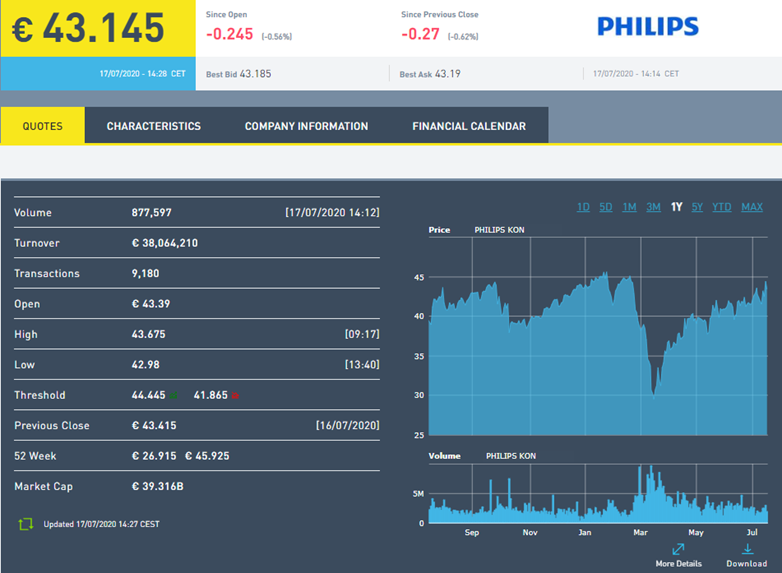
\includegraphics[width=0.85\textwidth]{philips.png}
\end{figure}
historical data yields estimated $\sigma=0.29$
\end{frame}

\begin{frame}{Example: put on Philips}
\vspace{.7cm}
\begin{figure}
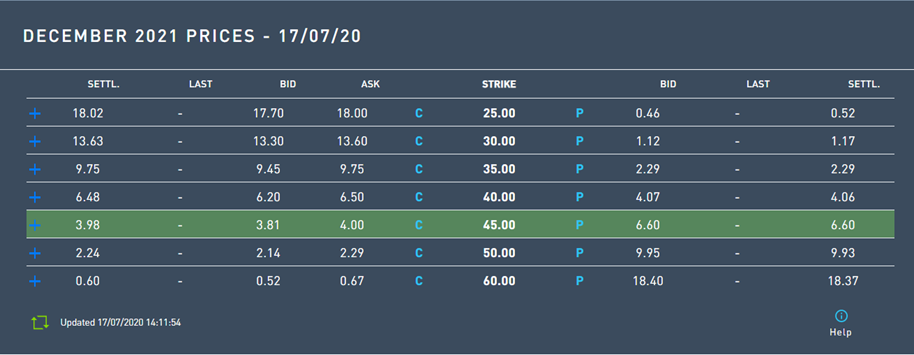
\includegraphics[width=\textwidth]{philips2.png}
\end{figure}
\begin{itemize}
\item
$T=17.5/12$, $r=0.01$, $K=45$, $\sigma=0.29$ and $S_0=43.145$ yields 6.70 as B-S price for the put,
where $\sigma=0.29$ is result from estimation on historical data on $S$.
\end{itemize}
\end{frame}

\section{Pricing Kernels}

\begin{frame}{Motivation}
\begin{itemize}
\item
suppose we work in standard Black-Scholes market with $B$ as num\'eraire
\item Girsanov yields probability measure $\mathbb{Q}$ defined by $\mathbb{Q}(A) = \mathbb{E}_{\mathbb{P}} 1_A Z_T$ where
\[
Z_t = \exp\left( - t (\mu-r)^2/(2\sigma^2) 
- ((\mu-r)/\sigma    ) W_t^{\mathbb{P}}
\right)
\]
\item we know 
$\mathbb{E}_{\mathbb{Q}}[ X ]
= \mathbb{E}_{\mathbb{P}}[ X Z_T ]$
\item it can be shown that
$\mathbb{E}_{\mathbb{Q}}[ X |\mathcal{F}_t]
= \mathbb{E}_{\mathbb{P}}[ X (Z_T/Z_t) |\mathcal{F}_t]$
\item we thus have
\begin{align*}
A_t 
&= \mathbb{E}_{\mathbb{Q}}\left[ \frac{N_t}{N_T} A_T \mid \mathcal{F}_t
\right]
=
\mathbb{E}_{\mathbb{P}}\left[ \frac{N_t}{N_T} \frac{ Z_T}{Z_t} A_T \mid \mathcal{F}_t
\right]
\end{align*}
which yields, with $K_t= Z_t / N_t$,
\[
K_t A_t  =\mathbb{E}_{\mathbb{P}}[ K_T A_T \mid
\mathcal{F}_t],
\]
i.e. $KA$ is a $\mathbb{P}$-martingale
\end{itemize}
\end{frame}

\begin{frame}{The first fundamental theorem of asset pricing (pricing kernel version)}
We proved, for the special case of the Black-Scholes market, the following theorem.
\begin{theorem}
Absence of arbitrage holds if and only if there exists a process $K$, with $K_t>0$, such that
for any asset with price $A_t$ the process $K_t A_t$ is a $\mathbb{P}$-martingale
\end{theorem}
\textbf{Application:}
\begin{itemize}
\item determine $K$ (using your models for the basic assets)
\item (no arbitrage) price of a derivative, with payoff $C_T$, based on these assets is given by
\[
C_t=\frac{1}{K_t}\mathbb{E}_{\mathbb{P}}[ K_T C_T \mid \calF_t]
\]
\end{itemize}

\end{frame}





\begin{frame}{The pricing kernel for the standard Black-Scholes world}
\small{
\begin{itemize}
\item try $K$ of the form
$
\rd K_t=\mu^K_t \rd t + \sigma^K_t \rd W_t
$
\item It\^{o}'s product rule yields
\begin{align*}
\rd K_t B_t&=K_t \rd B_t + B_t \rd K_t+ \rd [K,B]_t\\
&=( r K_t B_t + B_t \mu^K_t) \rd t + \ldots \rd W_t
\end{align*}
$K_tB_t$ martingale $\implies$ no drift $\implies$ $\mu^K_t=-rK_t$
\item
It\^{o}'s product rule yields
\begin{align*}
\rd K_t S_t&=K_t \rd S_t + S_t \rd K_t+ \rd [S,K]_t\\
&=\left(  K_t\mu S_t + S_t\mu^K_t+ \sigma \sigma^K_t S_t\right)   \rd t + \ldots \rd W_t
\end{align*}
$K_tS_t$ martingale $\implies$ no drift $\implies$ $\sigma^K_t=-K_t(\mu-r)/\sigma$
\end{itemize}
So
\[
K_0=1,\quad \rd K_t=-rK_t \rd t  -\frac{\mu-r}{\sigma} K_t \rd W_t
\]
determines the pricing kernel process in the B-S model.
}
\end{frame}
%
\begin{frame}{The pricing kernel for the standard Black-Scholes world}
\[
K_0=1,\quad \rd K_t=-rK_t \rd t  -\frac{\mu-r}{\sigma} K_t \rd W_t
\]
has as solution
\[
K_t=\exp\left\{
\left(-r-0.5\left(\frac{\mu-r}{\sigma}\right)^2 \right)t -\frac{\mu-r}{\sigma} W_t
\right\}
\]
Fair price of a derivative, with payoff $C_T=F(S_T)$, based on these assets is given by
\[
C_0=\frac{1}{K_0}\mathbb{E}_{\mathbb{P}}[ K_T C_T ]
\]
\begin{itemize}
\item $K_T C_T=g(W_T)f(S_T)=g(W_T)\tilde f(W_T)=h(W_T)$, so price determined by expectation of functional of $\rN(0,T)$ variable
\item price seems to depend on $\mu$, however it does not!
\end{itemize}
%$\implies$ price of claim with payoff $F_T(S_T)$ is given by
%\begin{align*}
%\mathbb{E} K_T F_T(S_T)&=
%\mathbb{E} \exp\left\{
%\left(-r-0.5\left(\frac{\mu-r}{\sigma}\right)^2 \right)T -\frac{\mu-r}{\sigma} W_T
%\right\} F_T( S_0\exp( (\mu-0.5\sigma^2)T +\sigma W_T))
%\\
%&=
%\exp\left\{
%\left(-r-0.5\left(\frac{\mu-r}{\sigma}\right)^2 \right)T
%\end{align*}
\end{frame}

\begin{frame}{Remark}
\begin{itemize}
\item you can always set $K_0=1$
\item which yields
\[
C_0 = \mathbb{E}_{\mathbb{P}}[ K_T C_T]
\]
\item
suppose $C_T = 1\{ \omega \in E\}$, i.e.
the pay-off is 1 euro in case event $E$ occurs
and 0 otherwise
\item
then
\[
C_0 = \mathbb{E}_{\mathbb{P}}[ 1_E K_T],
\]
so $K_T(\omega)$ kind of measures how
expensive it is to get a pay-off in state $\omega$
\item For the Black-Scholes market we have (assume
$\mu>r$)
\[
K_T=\exp\left\{
\left(-r-0.5\left(\frac{\mu-r}{\sigma}\right)^2 \right)T -\frac{\mu-r}{\sigma} W_T
\right\},
\]
showing that $K_T$ takes large values for large, negative values of $W_T$. And such state-of-the-world
correspond to small values of $S_T(\omega)$
\end{itemize}
\end{frame}



\section{Second Fundamental Theorem of
asset pricing}


\begin{frame}{Completeness}
In our discussion we have assumed that
it is possible to find a self-financing portfolio for every
option pay-off $C_T$. This property is referred to as `completeness'.
\\ 
\vspace{.5cm}
\textbf{Definition} \\
A financial market is said to be \textbf{complete} if it is possible
to find, for each $T>0$, and all random variables $C_T$ that are $\mathcal{F}_T$-measurable, a
self-financing portfolio $V$ (satisfying regularity conditions)
that satisfies $V_T=C_T$ (a.s.)
\end{frame}

\begin{frame}{Second Fundamental Theorem of asset pricing}
\textbf{Theorem} \\
Under regularity conditions we have:
a financial market 
is complete if and only if there is a \emph{unique}
measure $\mathbb{Q}\sim\mathbb{P}$ that makes 
all deflated asset prices $A/N$ $\mathbb{Q}$-martingales (where
$N$ is chosen num\'{e}raire.
\\
\vspace{.5cm}
\textbf{Examples}
\begin{itemize}
\item 
For our Black-Scholes market $\mathbb{Q}$ was unique, hence the
market is complete.
\item Consider the Black-Scholes market. Now we also add an additional risk factor to the market: an independent Brownian 
motion. This has impact on $\mathcal{F}_T$! And now claims could depend on both Brownian motions. No additional assets are available.  This leads to an incomplete market. (Why is
$\mathbb{Q}$ not unique?)
\end{itemize}
\textbf{Remark} In the MSc in QFAS we discuss
valuation (and hedging) in incomplete markets
(which you often encounter in case there is financial risk
as well as actuarial risk). 
\end{frame}


\end{document}